%$$$$$$$$$$$$$$$$$$$$$$$$$$$$$$$$$$$$$$$$$$$$$$$$$$$$$$$$$$$$$$$$$$$$$$$$$$$$$$$$
%Paragraph 1:Linux Scalability의 연구에 대한 설명
%$$$$$$$$$$$$$$$$$$$$$$$$$$$$$$$$$$$$$$$$$$$$$$$$$$$$$$$$$$$$$$$$$$$$$$$$$$$$$$$$

\newpage
\section{최근 운영체제 병렬화 연구}
\label{sec:osrelated}

%~\cite{Boyd-WickizerCorey}~\cite{Wentzlaff2010fOS}
%~\cite{Baumann2009Barrelfish}
%~\cite{Liu2009Tessellation}~\cite{Farrington2010Helios}

최근 병렬화 운영체제에 대한 연구는 새로운 확장성 있는 운영 체제를 만들거나 
기존 운영체제를 최적화 시키는 방향으로 연구가 진행되고 있다.
%~\cite{SilasBoydWickizer2010LinuxScales48}
%~\cite{AustinTClements2012RCUBalancedTrees}~\cite{Clements2013RadixVM}~\cite{SilasBoydWickizerPth}


\subsection{새로운 운영체제 제안}

\subsubsection{Corey}
Corey~\cite{Boyd-WickizerCorey}는 MIT의 PDOS(Parallel and Distributed Operating
Systems)에서 개발하였다.
Corey의 기본 철학은 커널 영역의 공유 데이터를 유저 응용프로그램이 사용할 수 있도록 인터페이스를 제공 함에 따라,
공유 데이터 때문에 발생하는 경합 문제를 유저 응용프로그램이 해결할 수 있도록 하는 방법을 사용하였다.
Corey가 이러한 방법을 사용한 이유는 매니코어 시스템에서는 코어 간의 캐시 일관성 작업 
때문에 성능이 저하되고, 이 현상이 발생하는 근본 원인이 운영체제가 응용프로그램의 특성에 관계 없이 
불필요하게 데이터를 공유하기 때문이다.
또한 하드웨어 역시 응용프로그램의 특성에 상관없이 캐시 메모리를 동기화 하는 방식을 사용하기 때문에,
기존 운영체제에서 취하는 방법을 사용하면 공유 문제를 해결 할 수 없다는 것이다.  
즉 기존 해결 방법들은 매니코어 환경에서 응용프로그램 특성에 따라 최적화 할 수 없다는 문제점을 가진다. 
이러한 문제를 해결하기 위해, Corey는 응용프로그램의 워크로드에 따라 공유 문제를 응용프로그램 작성자가 
직접 해결할 수 있는 방법을 제공해준다.
이러한 방법은 과거 연구되어온 커널의 자원을 유저와 공유할 수 있는 Exokernel~\cite{Engler1995EOS}의 개념을 가져와 
매니코어 시스템에 적용한 방법이며, Corey는 Exokernel의 개념을 통해 확장성을 개선하였다.


\begin{figure}[h!]
    \centering
    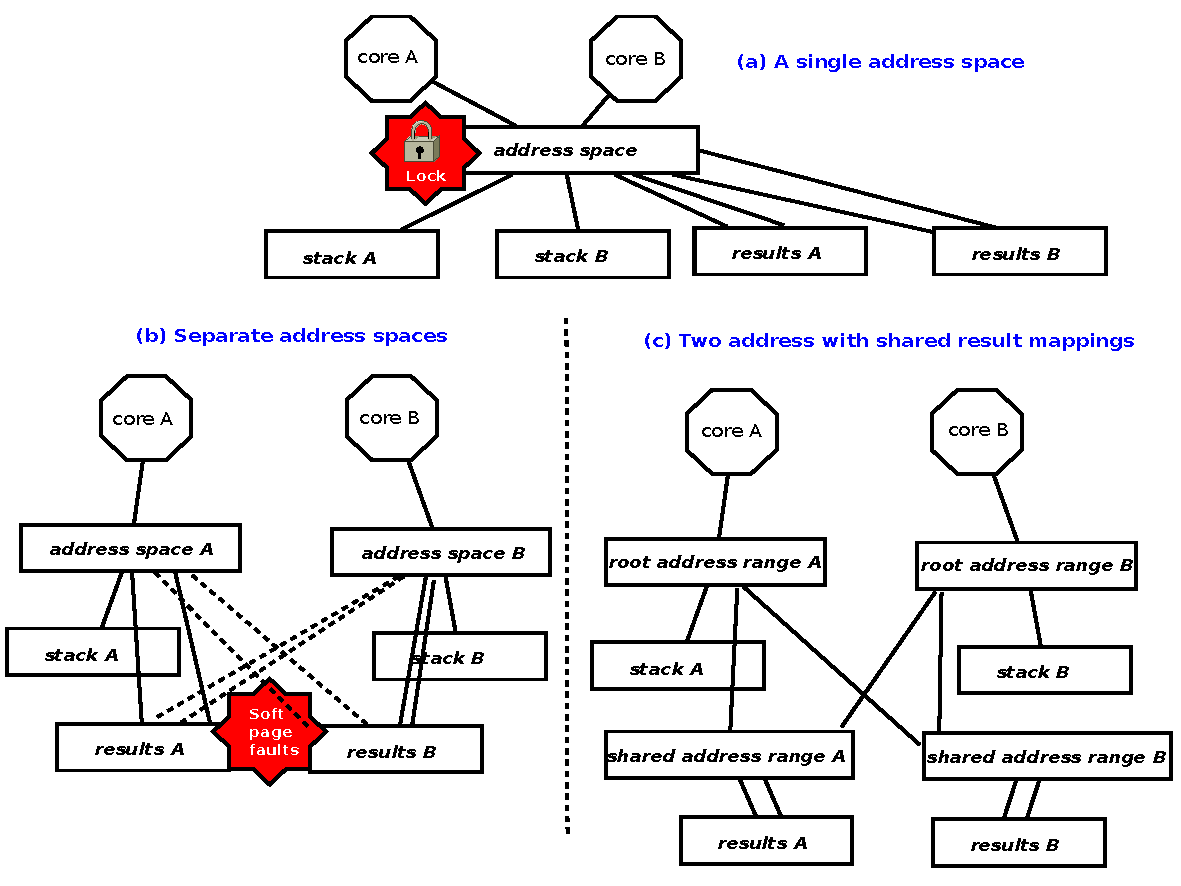
\includegraphics[width=1\textwidth]{fig/corey/corey}
    \caption{Corey 운영체제 address space 공유 방법}
  \label{fig:corey}
\end{figure}

%$$$$$$$$$$$$$$$$$$$$$$$$$$$$$$$$$$$$$$$$$$$$$$$$$$$$$$$$$$$$$$$$$$$$$$$$$$$$$$$$
%Paragraph 2:Corey의 3가지 기본 개념 설명
%$$$$$$$$$$$$$$$$$$$$$$$$$$$$$$$$$$$$$$$$$$$$$$$$$$$$$$$$$$$$$$$$$$$$$$$$$$$$$$$$
Corey는 3가지 기본적인 개념(Address Rages, Kernel Core, Shares)을 가지고 있다. 
첫째, Address Rages는 운영체제에서 여러 스레드간의 공유하는 데이터인 Address Space에 대해서 다룬다.
대부분의 운영체제는 Address Space를 그림~\ref{fig:corey}(a)와 같이 Single Address Space로
구성하는 경우 또는 그림~\ref{fig:corey}(b)와 같이 퍼코어 기반의 Separate Address Space로 구성하는 경우로
구성된다. 
만약 Single Address Space를 사용할 경우 모든 코어가 같은 Address Space를 공유함에 따라 반드시 락이
필요하고 이 락 때문에 스레드들이 직렬화된다.
예를 들어, 맵리듀스(MapReduce)와 같은 응용프로그램을 사용할 경우 맵 단계에서 굉장히 많은 락 경합이 발생하게 된다.
반대로, Separate Address Space를 사용할 경우 리듀스 단계에서 공유하지 않은 데이터에 접급함에 따라 
소프트 페이지 폴트(Soft Page Fault)가 많이 발생하는 문제가 발생한다.
Corey는 이러한 문제를 Address Rages라는 새로운 개념으로 해결하였다. 
이것은 그림~\ref{fig:corey}(c)와 같이 Separate Address Space를 제공함과 동시에 중간 결과를 공유할 수 있는
방법인 Single Address Space를 제공함에 따라, 두 장점을 동시에 취한다.
다음으로, Kernel Core는 응용프로그램의 공유 메모리를 사용하지 않고, 특정 코어에 
독점 할당 시켜주고 공유는 IPC로 하도록한 기술이다. 
따라서 스케줄러와 인터럽트에 방해를 받지 않고 캐시 지역성을 높여 성능을 향상 시킨다. 
마지막으로, 공유는 Exokernel과 같이 커널 자료구조를 응용프로그램에게 접근할 수 있는 
기능을 제공해준다.


\subsubsection{Barrelfish}

%$$$$$$$$$$$$$$$$$$$$$$$$$$$$$$$$$$$$$$$$$$$$$$$$$$$$$$$$$$$$$$$$$$$$$$$$$$$$$$$$
%Paragraph : Barrelfish의 특징 설명
%$$$$$$$$$$$$$$$$$$$$$$$$$$$$$$$$$$$$$$$$$$$$$$$$$$$$$$$$$$$$$$$$$$$$$$$$$$$$$$$$
Barrelfish~\cite{Baumann2009Barrelfish}는 취히리의 ETH와 마이크로 소프트(Microsoft)가
공동 연구하여 만든 운영체제이다.
Barrelfish는 멀티커널(Multikernel) 운영체제 중 하나 이고, 기본적인 철학은 공유 메모리 시스템 
기능들을 분산 처리 방식으로 구현하는 것이다.
예를 들어, 운영체제에서 각 코어는 마치 네트워크로 분산 된 시스템으로 가정하고, 서로 다른 코어 간에는 메시지 
패싱을 통해 통신을 하여 성능을 향상 시키는 방법이다. 
이러한 방법을 사용한 이유는 캐시 구조로 된 시스템의 단일화된 인터커넥트가 코어가 증가할 수록 캐시 
일관성 트래픽 문제를 야기 하기 때문에, 메시지 패싱 방법이 하나의 인터커넥트를 이용하는 하드웨어 캐시 일관성 
프로토콜을 사용하는 방법보다 오히려 더 높은 성능을 보이기 때문이다. 

%$$$$$$$$$$$$$$$$$$$$$$$$$$$$$$$$$$$$$$$$$$$$$$$$$$$$$$$$$$$$$$$$$$$$$$$$$$$$$$$$
%Paragraph : Barrelfish의 구조 설명 
%$$$$$$$$$$$$$$$$$$$$$$$$$$$$$$$$$$$$$$$$$$$$$$$$$$$$$$$$$$$$$$$$$$$$$$$$$$$$$$$$
이러한 Barrelfish의 구현은 그림~\ref{fig:Barrelfish}과 같다.
커널 레벨에서는 하드웨어와 밀접한 CPU Driver가 하드웨어 인터페이스를 제공한다.
CPU Driver는 유저 레벨의 모니터(Monitor)와 함께 하나의 운영체제 처럼 동작하며, 
이것은 마치 각 코어에 하나의 운영체제가 동작하는 것 처럼 보이는 멀티커널(Multikernel)의 구조를 따른다.
응용프로그램은 여러 코어를 이용할 수 있는데, 이러한 환경을 제공하기 위해 존재하는 것이 모니터이다. 
모니터는 운영체제의 기본 기능을 제공하기 위해 존재하며, 공유 메모리를 사용하기 
보다는 복제(Replication)와 IPC와 같은 분산 시스템에서 사용하는 방법을 이용한다. 
모니터는 View라는 상태를 가지고 복제를 수행한다. 
이러한 방법 공유 메모리 시스템을 분산 시스템에서 사용하는 방식과 같이 시스템을 구성하여, 
캐시 커뮤니케이션 때문에 발생하는 시스템 인터커넥트의 로드를 줄일 수 있다.

\begin{figure}[h!]
    \centering
    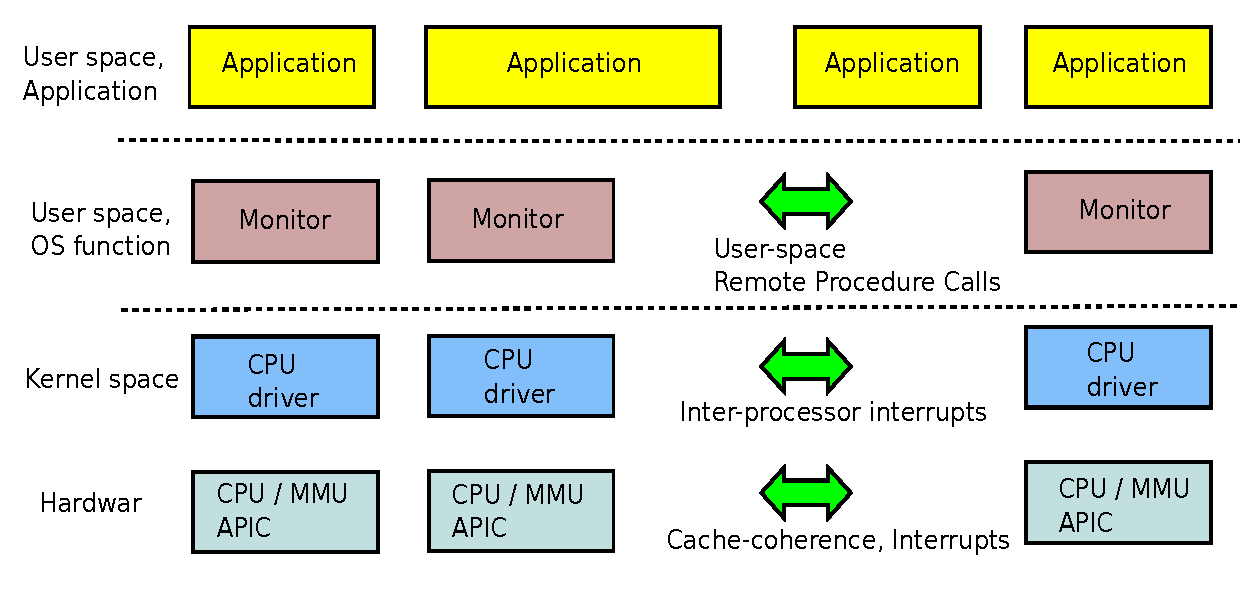
\includegraphics[width=1\textwidth]{fig/multikernel/multikernel}
    \caption{Barrelfish 구조}
  \label{fig:Barrelfish}
\end{figure}

%$$$$$$$$$$$$$$$$$$$$$$$$$$$$$$$$$$$$$$$$$$$$$$$$$$$$$$$$$$$$$$$$$$$$$$$$$$$$$$$$
%Paragraph : Barrelfish의 구조의 단점
%$$$$$$$$$$$$$$$$$$$$$$$$$$$$$$$$$$$$$$$$$$$$$$$$$$$$$$$$$$$$$$$$$$$$$$$$$$$$$$$$
Barrelfish의 단점은 Barrelfish의 구조적인 철학이 공유를 최대한 줄이는 것인데, 
이로 인해 로드 밸런싱을 수행할 수 없는 단점을 가져온다. 
예를 들어 하나의 코어에 여러 스레드들이 같이 돌고 있고, 다른 코어에는 아무런 
스레드도 없는 경우, Barrelfish는 분산 시스템 처럼 수행되므로 동적으로 스레드에 대한 정보들을 
다른 코어로 전송할 수가 없다.
즉 로드 밸런싱이 어려우므로 응용프로그램에 따라,
로드가 한 쪽에 몰리는 경우, 느려진 코어의 스레드들을 기다려야 하기 때문에 전체적인 
성능이 저하된다.  

\subsubsection{FusedOS}
%$$$$$$$$$$$$$$$$$$$$$$$$$$$$$$$$$$$$$$$$$$$$$$$$$$$$$$$$$$$$$$$$$$$$$$$$$$$$$$$$
%Paragraph : Fused OS의 특징 설명
%$$$$$$$$$$$$$$$$$$$$$$$$$$$$$$$$$$$$$$$$$$$$$$$$$$$$$$$$$$$$$$$$$$$$$$$$$$$$$$$$
FusedOS는 IBM 연구소에서 개발되었으며, 모노리틱 구조와 마이크로 구조를 혼합한 운영체제이다.
기존 연구들은 모두 경량 커널(LWK: Light-Weight Kernel) 또는 정량 커널(FWK:
Full-Weight Kernel) 둘 중 하나의 방식으로만 개발되었으나, 이 두가지를 
혼합하여 만든 운영체제이다.
이처럼 혼합하여 만든 운영체제인 FusedOS의 장점은 LWK를 통하여 FWK이 가지고 있는 근본적인 확장성 
문제를 해결함과 동시에, 과학에서 많이 사용되는 특정한 목적으로 개발된 응용프로그램을 
LWK에서 동작시킴에 따라 커널의 간섭이 없이 동작 시킬 수 있다는 것이다. 
또한, FWK의 장점 중 하나인 리눅스로 인하여 기존 만들어진 라이브러리들을 
리눅스의 장점을 모두 활용 할 수 있다.
 
\begin{figure}[h!]
    \centering
    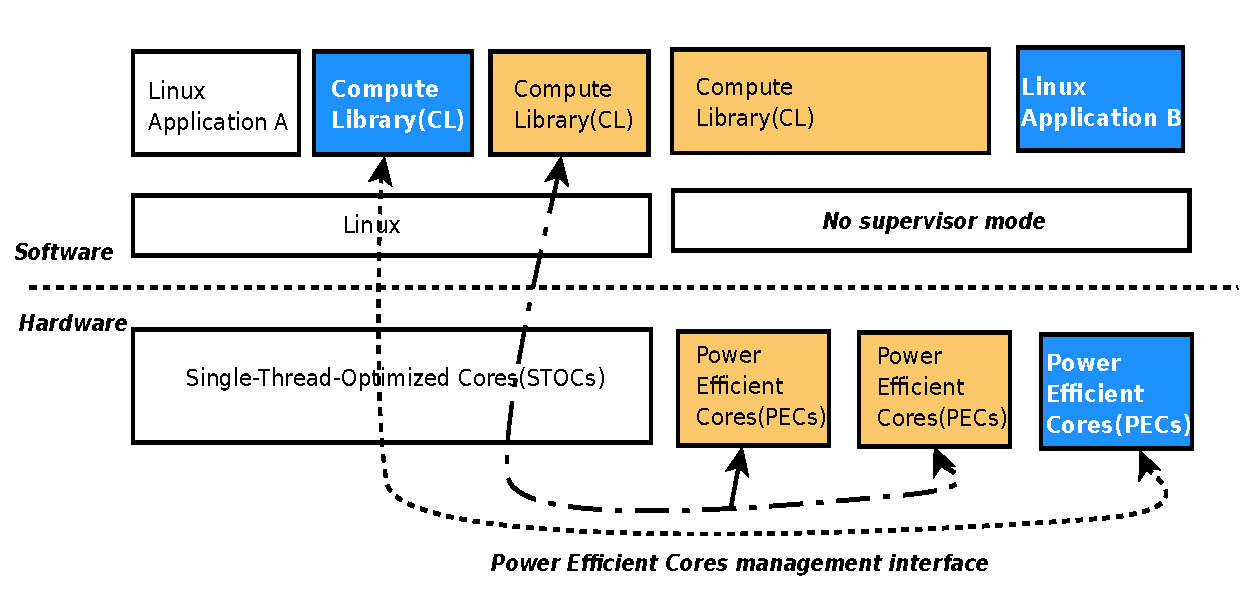
\includegraphics[width=1\textwidth]{fig/fusedos/fusedos}
    \caption{FusedOS 구조}
  \label{fig:FusedOS}
\end{figure}

%$$$$$$$$$$$$$$$$$$$$$$$$$$$$$$$$$$$$$$$$$$$$$$$$$$$$$$$$$$$$$$$$$$$$$$$$$$$$$$$$
%Paragraph : Fused OS의 구조 설명
%$$$$$$$$$$$$$$$$$$$$$$$$$$$$$$$$$$$$$$$$$$$$$$$$$$$$$$$$$$$$$$$$$$$$$$$$$$$$$$$$
이러한 FusedOS의 구조는 그림~\ref{fig:FusedOS}과 같다. 
그림과 같이 FusedOS의 하드웨어는 성능 좋은 코어 그룹(STOCs: Single-Thread-Optimized Cores)과
전력에 효율적인 코어 그룹(PECs: Power Efficient Cores)으로 구성되어 있다.
PEC는 STOC의 기능 중 하나이나 관리자(Supervisor) 모드를 포함하고 있지는 않는다. 
STOC에는 리눅스 운영체제가 동작하고, 기존 리눅스에 기능을 추가하여 Compute Library(CL)이 PEC에 
접근이 가능하도록 설계되었다.

CL은 마치 리눅스 응용프로그램처럼 동작하며, 실행이 되면 다음으로 가벼운 커널을 PEC 커널 쪽 메모리에 
전달하고 그 후 가벼운 커널은 PEC 코어에서 동작하게 된다.
이러한 구조를 통해, HPC 응용의 성능을 보여주면서 리눅스 운영체제의 기능을 제공할 수 있는 장점을 가진다. 
FusedOS의 성능은 HPC 운영체제 코어와 연산을 위한 코어가 분리되었기 때문에, 운영체제의 
방해를 받지 않아 기존 리눅스보다 높은 성능을 보인다.
이것을 통해 기존 운영체제의 병목 현상인 캐시 일관성 유지 때문에 발생하는 확장성 문제를 해결할 수 있다.
하지만 FusedOS의 문제점은 독립적으로 코어에 LWK를 할당하여 호출하는 방법을 사용하므로,  
응용프로그램을 실행하고 종료하는데 추가적인 시간을 가지는 단점이 있다.

\subsection{기존 운영체제 최적화}

\subsubsection{Linux Scalability}

앞에서 설명한 새로운 운영체제에 대한 연구 뿐만 아니라 기존 운영체제의 확장성에 대한 연구가 진행되었다. 
특히 MIT PDOS 연구 그룹은 새로운 운영체제가 아닌 리눅스 커널을 대상으로 매니코어 환경에서 확장성을 연구하였다.
실제 많이 사용되는 7가지의 응용프로그램(Exim, Memcached, Apache, PostgreSQL, Gmake, Psearchy,
MapReduce)을 가지고 MOSBENCH라는 응용프로그램 벤치마크를 만들어 리눅스 커널을 대상으로 실험을 
하였고, 측정 중 발생되는 여러 문제를 해결하여, 종합적인 리눅스 커널의 확장성을 향상시켰다.

\begin{figure}[h!]
    \centering
    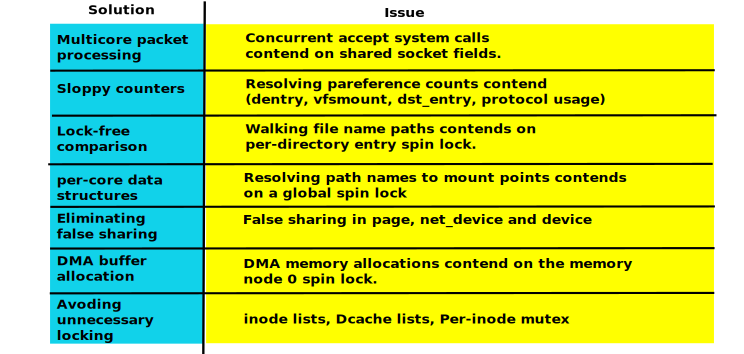
\includegraphics[width=1\textwidth]{fig/linux/linux}
    \caption{Linux scalability 분석 연구}
  \label{fig:linux}
\end{figure}

이 연구는 그림~\ref{fig:linux}과 같이 총 7가지의 기술을 활용하였고, 추가적으로 응용프로그램을 직접 수정하여 
커널의 확장성을 개선하였다.
이러한 7가지 기술 중 하나는 멀티코어 패킷 프로세싱이 있다. 
그 동안 리눅스 커널은 네트워크 멀티코어 패킷에 대해서 멀티 큐를 사용하여 성능과 확장성을 이루었으나, 
클라이언트 연결 주기가 짧을 경우 이러한 방법도 여전히 성능과 확장성 문제를 가진다.
따라서 이 연구 그룹은 아파치(Apache) 응용프로그램과 같이 동시 다발 적으로 연결을 요청하는 경우 
퍼코어 큐에 저장하도록 \code{accpet()}을 수정하였다. 
이 것은 싱글 리스닝(Listening) 소켓을 보호하기 위해 존재하는 락을 제거할 수 있으므로 확장성을 향상 시킨다.

다음으로 이 연구 그룹은 리눅스의 참조 카운터 때문에 발생하는 캐시 일관성 트래픽을 제거하기 위해 
\textit{sloppy counter}를 만들었다.
그리고 이 \textit{sloppy counter}를 디렉터리 엔트리 오브젝트(\code{dentrys}), 마운트된 파일 시스템
오브젝트(\code{vfsmounts}) 그리고 네트워크 프로토콜에서의 메모리 할당을 추적하기 위한 전역 변수에 
적용하여 성능 및 확장성을 향상 시켰다.
또한 리눅스 커널은 디렉토리 엔트리 캐시의 이름을 찾는 부분에 \textit{per-dentry spin lock} 때문에 문제가 
있는데, 이 문제를 해결하기 위해 리눅스의 \textit{lock-free page-cache lookup protocol}과
유사한 방법을 만들어 전역 \textit{spin lock}을 제거하였다.
그 이외에도 퍼코어 방법을 사용한 방법과 캐시 라인의 \textit{false sharing} 때문에 발생하는 성능 저하 문제, 
이더넷 디바이스 DMA 버퍼가 한쪽 노드에만 할당되어 발생하는 확장성 문제와 그리고 불필요한 락을 
제거하여 리눅스 커널의 확장성을 향상 시켰다.  

\subsubsection{BonsaiVM}
%$$$$$$$$$$$$$$$$$$$$$$$$$$$$$$$$$$$$$$$$$$$$$$$$$$$$$$$$$$$$$$$$$$$$$$$$$$$$$$$$
%Paragraph : BonsaiVM 특징 설명
%$$$$$$$$$$$$$$$$$$$$$$$$$$$$$$$$$$$$$$$$$$$$$$$$$$$$$$$$$$$$$$$$$$$$$$$$$$$$$$$$
BonsaiVM은 MIT PDOS에서 개발한 리눅스 커널을 위한 가상 메모리 관리 시스템이다. 
리눅스의 멀티 스레드들은 하나의 Address Space를 공유하게 되는데, 이러한 공유된 Address Space을 사용하는 
스레드들은 \code{mmap/munmap}과 소프트 페이지 폴트간에 락 경합을 발생 시킨다.
리눅스는 공유된 Address Space를 보호하기 위해, 락 경합 중 블락킹 동기화 기법 중 하나인
읽기-쓰기(reader-writer) 세마포어를 사용하여 보호한다.
이러한 동기화 기법을 사용함에 따라, Address Space를 때문에 여러 스레드들이 블락 걸리는 현상이 많이 발생하는데, 
이 때문에 결국 코어가 많아져서 여러 스레드가 같은 Address Space에 접근하면서 Single Address Space 문제가
발생하여 성능이 저하된다.

\begin{figure}[h!]
    \centering
    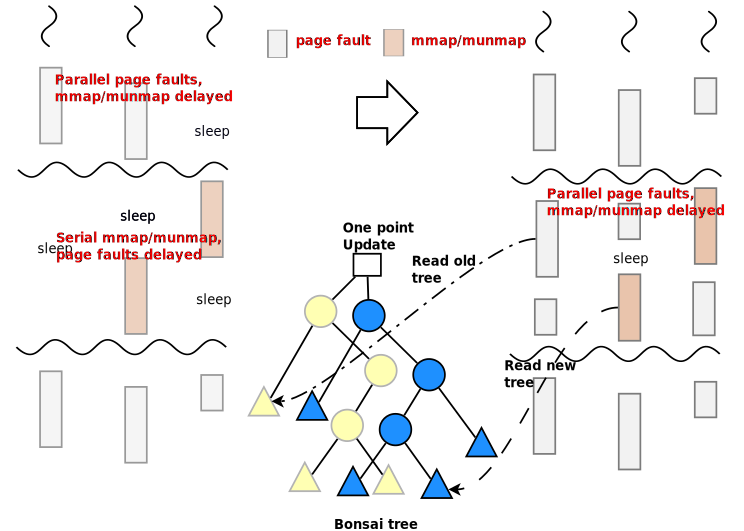
\includegraphics[width=1\textwidth]{fig/bosaivm/bosaivm}
    \caption{Address space 문제와 BosaiVM을 이용한 해결}
  \label{fig:bonsaivm}
\end{figure}

그림~\ref{fig:bonsaivm}의 왼쪽 부분은 이러한 Address Space의 문제를 보여준다. 
병렬로 수행이 가능한 페이지 폴트 때문에 \code{mmap/munmap} 함수에 의해 스레드들은 블락이 걸리고, 병렬로 
수행이 불가능한 \code{mmap/munmap} 함수가 수행되면, \code{mmap/munmap} 함수 뿐만 아니라 
페이지 폴트가 발생한 스레드들까지 블락에 걸린다.
이러한 Single Address Space 문제를 해결하기 위해, 앞에서 설명한 Corey 운영체제와 같이 새로운 운영체제를 
만드는 등 여러 연구들이 진행되었지만, 이 연구에서는 기존 리눅스 커널을 대상으로 구현하였다.
방법은 동기화 기법 중 하나인 RCU와 새로운 밸런스 트리(\code{Bonsai})를 이용하여 Single Address Space 문제를
해결하였다.
즉 리눅스 커널을 대상으로 확장성을 개선한 연구이며, 
리눅스 커널 중 상당히 복잡한 가상 메모리 시스템에 직접 RCU라는 동기화 기법을 적용하여, 
성능 확장성을 향상 시킨 연구이다.
 
BonsaiVM은 총 3가지 기법(\textit{fault locking, hybrid locking/RCU, pure RCU})을 통해
Single Address Space 문제를 해결하였다.
이 중 앞의 두 가지 방법은 리눅스 커널의 구현 의존 적인 해결 방법이고, \textit{pure RCU}는 
기존 리눅스 커널의 레드-블랙 트리를 사용하지 않고 RCU를 사용할 수 있는 
새로운 \code{Bonsai} 트리 자료구조를 만들어 문제를 해결한 방법이다. 
\code{Bonsai} 트리는 그림~\ref{fig:bonsaivm}와 같이 이진 트리로 구성되어 있다. 
\code{Bonsai} 트리의 가장 큰 특징은 루트 노드의 업데이트가 원자적 명령으로 한번에 이루어 진다는 것이다. 
그 이유는 Bonsai 트리는 함수형 트리 형식으로 개발되어서, 밸런스를 수행하는 동안에도 읽기 연산들은 
오래된 트리의 값을 읽을 수 있으며, 병렬로 수행할 수 있는 장점을 가진다는 것이다.
즉 RCU의 장점을 활용하여 여러 읽기 연산과 한가지의 쓰기 연산을 수행하는 스레드들을 병렬로 수행할 수 
있는 장점을 가진다. 
하지만 \code{Bonsai} 트리는 여러 스레들간에 경쟁이 발생하지 않는 경우, 트리 검색이 기존 레드-블랙 트리에 비해 많은 성능 
오버헤드를 가지는 문제점이 있다. 
 
%$$$$$$$$$$$$$$$$$$$$$$$$$$$$$$$$$$$$$$$$$$$$$$$$$$$$$$$$$$$$$$$$$$$$$$$$$$$$$$$$
%Paragraph 2: 기법 설명
%$$$$$$$$$$$$$$$$$$$$$$$$$$$$$$$$$$$$$$$$$$$$$$$$$$$$$$$$$$$$$$$$$$$$$$$$$$$$$$$$

\subsubsection{RadixVM}

%$$$$$$$$$$$$$$$$$$$$$$$$$$$$$$$$$$$$$$$$$$$$$$$$$$$$$$$$$$$$$$$$$$$$$$$$$$$$$$$$
%Paragraph : RadixVM 특징 설명
%$$$$$$$$$$$$$$$$$$$$$$$$$$$$$$$$$$$$$$$$$$$$$$$$$$$$$$$$$$$$$$$$$$$$$$$$$$$$$$$$
RadixVM은 BosaiVM과 같은 연구 그룹이 수행한 연구이며, 
Single Address Space 때문에 발생하는 확장성 문제를 해결하기 위해, 연구 용 운영체제인 sv6의 가상 메모리에 
대한 부분을 수정하여 Single Address Space 문제를 해결한 연구이다.
그 이유는 리눅스의 가상 메모리를 수정하는 것은 굉장히 복잡하여 리눅스 커널에 직접 적용하기에는 힘든 문제점이 
있기 때문에, 상대적으로 덜 복잡한 sv6 운영체제에 새로운 개념인 RadixVM을 적용하였다. 
RadixVM은 BonsaiVM과 같이 가상 메모리 시스템에서 공유되는 Address Space가 \code{mmap, unmap, page
fault} 함수 들로 인해 서로 경쟁함으로 발생하는 문제를 3가지 접근을 통해 해결하였다. 

\begin{figure}[h!]
    \centering
    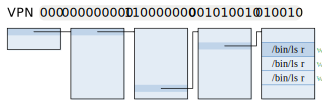
\includegraphics[width=1\textwidth]{fig/radix/radix}
    \caption{RadixVM의 해결 방법}
  \label{fig:radix}
\end{figure}

%$$$$$$$$$$$$$$$$$$$$$$$$$$$$$$$$$$$$$$$$$$$$$$$$$$$$$$$$$$$$$$$$$$$$$$$$$$$$$$$$
%Paragraph : RadixVM  기법 설명 - 1
%$$$$$$$$$$$$$$$$$$$$$$$$$$$$$$$$$$$$$$$$$$$$$$$$$$$$$$$$$$$$$$$$$$$$$$$$$$$$$$$$
첫째, 기존 밸런스 트리를 사용하지 않고, 기수(\code{Radix}) 트리를 이용하는 것이다. 
그 이유는 RadixVM의 궁극적인 목적은 가상 메모리와 관련된 연산에 대해서 최대한 공유를 피하자는 것이다, 
가장 쉬운 방법으로는, 모든 메모리 맵을 배열로서 만들면 모든 가상 메모리 관련 연산들의 충돌은 일어나지 않기 때문에 
쉽게 해결된다.
하지만 단순히 배열을 이용한 방법은 너무 많은 메모리 사용량이 요구된다.
메모리 오버헤드 문제를 해결하기 위한 가장 좋은 방법은 하드웨어 페이지 테이블처럼 동작하는 
기수 트리를 이용하는 것이다.
이처럼 기수 트리는 트리의 읽기와 쓰기 연산을 메모리의 서로 다른 부분에 접근하도록 만들어 준다.
따라서 배열을 사용한 방법과 같이 충돌 없이 사용 가능함과 동시에 메모리 오버헤드도 함께 줄일 수 있다.
결론적으로 여러 스레드들이 접근 할 수 있을 뿐 만아니라 메모리 사용량도 밸런스 트리와 비슷한 
수준을 유지 할 수 있는 장점을 가진다.

%$$$$$$$$$$$$$$$$$$$$$$$$$$$$$$$$$$$$$$$$$$$$$$$$$$$$$$$$$$$$$$$$$$$$$$$$$$$$$$$$
%Paragraph : RadixVM  기법 설명 - 2
%$$$$$$$$$$$$$$$$$$$$$$$$$$$$$$$$$$$$$$$$$$$$$$$$$$$$$$$$$$$$$$$$$$$$$$$$$$$$$$$
\code{RadixVM}의 두번째 기법은 \code{munmap}할 때 발생하는 \textit{TLB shutdown} 문제를 해결 한다.
이러한 \textit{TLB shutdown} 문제가 발생하는 이유는 다음과 같다. 
\code{unmap} 함수는 반드시 어떠한 코어의 페이지도 
매핑이 안된 상태로 끝나야 하는데, 이를 유지하기 위해 \code{unmap}
함수는 모든 코어에 \textit{TLB shutdonw} 메시지를 남긴다.
결국 코어가 증가 할 수록 모든 코어에
\textit{TLB shutdown} 메시지를 발생 시키므로 성능 문제가 발생 된다.
\code{RadixVM}에서는 이러한 \textit{TLB shutdown} 문제를 퍼코어 페이지 테이블을 이용하여 해결하였다. 

%$$$$$$$$$$$$$$$$$$$$$$$$$$$$$$$$$$$$$$$$$$$$$$$$$$$$$$$$$$$$$$$$$$$$$$$$$$$$$$$$
%Paragraph : RadixVM  기법 설명 - 2
%$$$$$$$$$$$$$$$$$$$$$$$$$$$$$$$$$$$$$$$$$$$$$$$$$$$$$$$$$$$$$$$$$$$$$$$$$$$$$$$
\code{RadixVM}의 마지막 기법은 새로운 \code{refcache}라는 레퍼런스 카운터(Reference Counter)이다. 
실제 운영체제에서 레퍼런스 카운터는 가장 큰 확장성 저해요소 중에 하나이다.
그 이유는 레퍼런스 카운터는 많은 캐시 일관성 트래픽을 발생 시키기 때문이다.
이러한 레퍼런스 카운터는 기본적으로 3가지 종류로 개발되고 있다. 
먼저 가장 쉬운 방법인 락을 이용하는 방법이 있다. 
즉 모든 증가/감소 명령의 앞뒤에 락을 호출하는 것이다. 
이것은 락 때문에(락 자체가 전변 변수를 이용) 상당히 많은 캐시-라인 경합이 발생된다. 
다른 방법으로는 원자적 증가/감소 명령을 이용하는 것이다. 
하지만 이러한 방법도 결국 전역 변수 때문에 캐시-라인 경합이 발생한다. 
최근의 방법으로는 파티션닝 기법 중 하나인 퍼코어 카운터를 이용하는 것이다. 
하지만, 단순히 퍼코어 카운터를 이용하는 것은 코어 수에 비례하여 공간에 대한 오버헤드를 가지게 된다.
\code{RadixVM}은 이러한 확장성과 메모리 사용량에 대한 오버헤드를 동시에 줄이기 위해, 
특정 시간(Epoch, 10ms)을 기반으로 퍼코어에 저장된 델타 카운트를 
주기적으로 체크하여 퍼코어에 저장된 카운터의 상태를 보고 전역 카운터에 적용하는 방법을 사용한다.
이 방법은 확장성을 높일 수 있을 뿐만 아니라, 동시에 공간에 대한 오버헤드를 줄인다. 

\subsubsection{Scalable Commutativity Rule}

%$$$$$$$$$$$$$$$$$$$$$$$$$$$$$$$$$$$$$$$$$$$$$$$$$$$$$$$$$$$$$$$$$$$$$$$$$$$$$$$$
%Paragraph : SC rule 특징 및 역사 설명 
%$$$$$$$$$$$$$$$$$$$$$$$$$$$$$$$$$$$$$$$$$$$$$$$$$$$$$$$$$$$$$$$$$$$$$$$$$$$$$$$$
SC Rule(Scalable Commutativity Rule)은 MIT PDOS 연구 그룹에서 운영체제의 확장성 개선을 위해 새로운
관점으로 바라본 연구이다.
기존 연구들은 대부분 운영체제의 병목지점을 추출한 후 발견된 병목지점을 해결하기 위해 새로운 
동기화 기법을 개발하거나 기존 개발된 동기화 기법을 적용하는 방법을 이용했다. 
하지만, 이러한 방법들은 모두 워크로드가 다름에 따라 서로 다른 결과를 가지게 되고, 
또한 문제를 해결하는데도 너무 많은 시간이 소요된다는 문제점을 가지고 있다.
실제 확장성에 대한 문제는, 대부분 설계 단계에서 해결 할 수 있으며, 설계 인터페이스를 확장성 있게 만들면, 
확장성 있는 시스템을 쉽게 만들 수 있다는 것을 주장하였다.
그 이유는 기존 개발되어온 운영체제(예를 들어 리눅스)는 응용프로그램이 커널의 자원을 
확장성 있게 사용하면 확장성에 문제가 해결 되기 때문이다. 
따라서, 확장성 있는 설계가 중요하며, 이를 위해 SC Rule은 리눅스 시스템 콜 연산에 대한 가환성(Commutativity)을 정의하였고, 
그에 대한 이론을 설명하였다.
가환성을 예를 들어 설명하면, 원자적으로 값 X를 변수 A에 추가하고, 
다른 CPU가 원자적으로 같은 변수에 Y라는 값을 추가하였다면, 
두 가지의 명령은 순서가 상관이 없고, 결국에는 X + Y의 값이 변수 A에 저장된다는 것이다.
이러한 수학적인 가환성을 리눅스의 시스템 콜을 대상으로 적용하였으며, 새로운 가환성을 정의 하였다.

%$$$$$$$$$$$$$$$$$$$$$$$$$$$$$$$$$$$$$$$$$$$$$$$$$$$$$$$$$$$$$$$$$$$$$$$$$$$$$$$$
%Paragraph : SC rule 예제 설명 
%$$$$$$$$$$$$$$$$$$$$$$$$$$$$$$$$$$$$$$$$$$$$$$$$$$$$$$$$$$$$$$$$$$$$$$$$$$$$$$$$
저자는 SIM(State-dependent, Interface-based, Monotonic)라고 부르는 새로운
POSIX 운영체제의 가환성(commutativity)에 대해서 정의를 하였다.
또한 POSIX의 오퍼레이션에 대한 가환성을 여러 오퍼레이션을 예로 들며 설명하였다.
\code{open(``a'', O\_CREAT|O\_EXCL)}을 두 개의 코어가 같은 디렉토리에서 수행하면 가환성이 없는데, 
이것을 다른 디렉토리에서 수행하면 가환성을 가진다는 것이다.
저자가 주장하는 SIM 가환성은 시스템 콜 함수들을 구별할 수 있게 만들어주고, 결국 
인터페이스 레벨에서 가환성을 가짐에 따라 확장성 있는 시스템을 가질 수 있다는 것이다.  
또 다른 예로 프로세스를 복사하는 \code{fork()}는 가환성이 없는데, 
\code{fork()}를 \code{posix\_spawn()}으로 수정하면 가환성을 가지게 되고, 이것은 결국 
시스템의 확장성을 향상 시키게 된다. 
이러한 원리는 결국 앞에서 설명하였듯이, 리눅스는 응용프로그램의 방법에 따라 확장성을 가질 수 있다는 것을 
활용한 연구이며, 이 연구는 리눅스 특성들을 잘 이용한 연구이다. 
결국 리눅스 커널은 가환성을 잘 지키도록 호출 해주면, 확장성을 향상 시킬 수 있고 
이것은 설계 단계에서 처리가 가능하다는 것이다. 
또한 저자는 QEMU을 수정하여 리눅스의 가환성을 분석 할 수 있는 \code{Commuter}라는 툴을 제공한다. 
이러한 툴을 통해 설계 단계에서 확장성 문제를 발견할 수 있도록 하였으며, 이 툴을 통해 저자가 
직접 운영체제(리눅스, sv6)의 문제점을 분석하였다. 
